\documentclass[a4,landscape]{seminar}
%\usepackage[dvips]{pstcol}
%\usepackage[pdf]{pstricks}
\usepackage{fancybox,epsfig,graphicx,pifont,slashed,soul}
\usepackage{semcolor}
\usepackage{rotating}
\usepackage{semlayer}
\usepackage{changepage}
\usepackage{amsmath}
\usepackage{hyperref}
%\usepackage{semdem}
\input{seminar.bug}
%\HyperSetUp
% slide size
\addtolength{\slideheight}{4cm}
\addtolength{\slidewidth}{3cm}
% laptop style overlays
\makeatletter
\def\pst@initoverlay#1{%
\pst@Verb{%
/BeginOL {dup (all) eq exch TheOL le or {IfVisible not {Visible
/IfVisible true def} if} {IfVisible {Invisible /IfVisible false def} if}
ifelse} def
\tx@InitOL /TheOL (#1) def}}
\makeatother

% miscellaneous macros
\def\toinf#1{\mathrel{\mathop{\sim}\limits_{\scriptscriptstyle
{#1\rightarrow\infty }}}}
\def\tozero#1{\mathrel{\mathop{\sim}\limits_{\scriptscriptstyle
{#1\rightarrow0 }}}}
\def\toone#1{\mathrel{\mathop{\sim}\limits_{\scriptscriptstyle
{#1\rightarrow1 }}}}
\newcommand{\specialcell}[2][c]{%
  \begin{tabular}[#1]{@{}c@{}}#2\end{tabular}}
\newcommand{\prog}{{\magenta\ding{46}}}
\newcommand{\tick}{{\green\ding{52}}}
\newcommand{\cross}{{\red\ding{55}}}%------------------------------------
\newcommand{\aqq}{\alpha_s \left( Q^2_0 \right)}
\newcommand{\aq}{\alpha_s\left( Q^2 \right)}
\newcommand{\extra}{\mathrm{extra}}
\newcommand{\mrexp}{\mathrm{exp}}
\newcommand{\dat}{\mathrm{dat}}
\newcommand{\1}{1\!\!\!1}
\newcommand{\one}{\mathrm{(1)}}
\newcommand{\two}{\mathrm{(2)}}
\newcommand{\art}{\mathrm{art}} 
\newcommand{\rep}{\mathrm{rep}}
\newcommand{\net}{\mathrm{net}}
\newcommand{\lc}{\left[}
\newcommand{\rc}{\right]}
\newcommand{\la}{\left\langle}
\newcommand{\ra}{\right\rangle}
\newcommand{\lp}{\left(}
\newcommand{\rp}{\right)}
\def\gsim{\mathrel{\rlap{\lower4pt\hbox{\hskip1pt$\sim$}}
    \raise1pt\hbox{$>$}}}         %greater than or approx. symbol
\def\lsim{\mathrel{\rlap{\lower4pt\hbox{\hskip1pt$\sim$}}
    \raise1pt\hbox{$<$}}}         %less  than or approx. symbol
\def\sitontop#1#2{\mathrel{\mathop{\scriptstyle #1}\limits_{\scriptstyle #2}}}
\def\blan{\Big\langle}
\def\bran{\Big\rangle}
\def\lsim{\mathrel{\rlap{\lower4pt\hbox{\hskip1pt$\sim$}}
    \raise1pt\hbox{$<$}}}         %less than or approx. symbol
\def\wup{{W^+}}
\def\wum{{W^-}}
\def\wupm{{W^\pm}}
\def\wump{{W^\mp}}
\newcommand{\stw}{\mbox{$\sin^2\theta_W$}}
\newcommand{\nub}{\overline{\nu}}
\newcommand{\nue}{\nu_{e}}
\newcommand{\numu}{\nu_{\mu}}
\newcommand{\nubmu}{\overline{\nu_{\mu}}}
\newcommand{\nube}{\overline{\nu_{e}}}
\newcommand\as{\alpha_s} 
\def\tr{\,{\hbox{\rm tr}}\,}
\def\epm#1#2{\hbox{${\lower1pt\hbox{$\scriptstyle +#1$}}
\atop {\raise1pt\hbox{$\scriptstyle -#2$}}$}}
\def\wup{{W^+}}
\def\wum{{W^-}}
\def\wupm{{W^\pm}}
\def\wump{{W^\mp}}
\newcommand{\tot}{\mathrm{tot}}
\newcommand     \bea     {\begin{eqnarray}} 
\newcommand     \eea     {\end{eqnarray}} 
\newcommand     \beq     {\begin{equation}} 
\newcommand     \eeq    {\end{equation}} 
\newcommand{\NS}{\mathrm{NS}}
\renewenvironment{equation}{\begin{displaymath}}{\end{displaymath}}

% font and colour declarations
\DeclareFontFamily{OT1}{bookman}{}
\DeclareFontShape{OT1}{bookman}{m}{n}{ <-> pbklc}{}
\DeclareFontShape{OT1}{bookman}{bx}{n}{ <-> pbkdc}{}
\DeclareFontShape{OT1}{bookman}{m}{it}{ <-> pbkdli}{}
\pagestyle{empty}
\renewcommand{\familydefault}{bookman}
\newrgbcolor{grey}{0.2 0.2 0.2}
\newrgbcolor{orange}{1.00 0.65 0.00}
\newrgbcolor{purple}{0.63 0.13 0.94}
\newrgbcolor{darkgreen}{0.00 0.39 0.00}
\newrgbcolor{skyblue}{0.53 0.81 0.92}
\newrgbcolor{tomato}{1.00 0.39 0.28}
\newrgbcolor{coral}{1.00 0.50 0.31}
\newrgbcolor{brown}{0.72  0.52 0.04}
\newrgbcolor{gold}{1.00 0.84 0.00}
\begin{document}
% correction for 2nd level itemization font
\renewcommand{\labelitemii}{\textrm{--}}
% slide frame style
\slideframe{none}
%
% begin presentation
%


\begin{slide}
  \begin{minipage}{.47\linewidth}
\begin{flushleft}
\includegraphics[width=.48\linewidth,clip]{nnpdf_logo_official.pdf}\end{flushleft}
\end{minipage}
\begin{minipage}{.47\linewidth}\begin{flushright}

\includegraphics[width=.16\linewidth,clip]{LOGO-ERC.jpg}
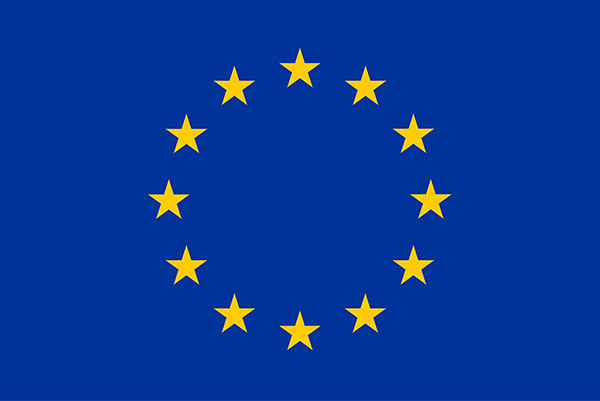
\includegraphics[width=.22\linewidth,clip]{flag_yellow_low.jpg}

\includegraphics[width=.51\linewidth,clip]{n3pdflogo_noback.png}
\end{flushright}\end{minipage}
%\hypersetup{pdfpagetransition=Dissolve}
\renewcommand{\slidestretch}{.8}
\begin{center}
\vspace{.6cm}
 {\bf\huge {\red THEORY AND METHODOLOGY:}}\\
\vspace{.4cm}
 {\bf\huge\darkgreen NEW DEVELOPMENTS}\\
\vspace{1. cm}
{\Large {\blue The NNPDF collaboration \& N3PDF TEAM}\\
 {\small Amsterdam-Barcelona-Cambridge-Edinburgh-Milan-NIKHEF}
}
%\end{center}
\vglue.8cm
\begin{minipage}{.49\linewidth}
\begin{flushleft}
  \vspace{.5cm}
{PDF4LHC meeting}
\end{flushleft}
\end{minipage}
\begin{minipage}{.49\linewidth}
\begin{flushright}
\vspace{.5cm}
{CERN, March 22, 2021} 
\end{flushright}
\end{minipage}
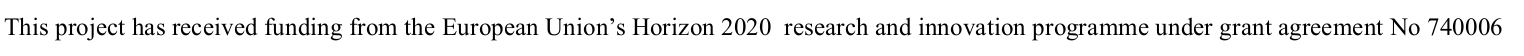
\includegraphics[width=.7\linewidth]{funding.png}
\end{center}
\end{slide}
\renewcommand{\slidestretch}{.7}
\begin{slide}{\small
\begin{center}{\large\darkgreen SUMMARY}\\
{\blue THEORY DEVELOPMENTS}
\end{center}
\begin{itemize}
\item  Electroweak Corrections   \qquad {\bf Christopher Schwan} (Milan)
\item Nuclear and deuteron corrections \qquad {\bf Rosalyn Pearson} (Edinburgh)
\end{itemize}
\begin{center}
{\blue PDF PROPERTIES AND THEIR IMPLEMENTATION}
\end{center}
\begin{itemize}
\item PDF positivity (TH) \qquad {\bf Felix Hekhorn} (Milan)
\item PDF basis, positivity (PH), integrability  \qquad
  {\bf Tommaso Giani} (NIKHEF)
\end{itemize}
\begin{center}
{\blue  PDF DETERMINATION METHODOLOGY}
\end{center}
\begin{itemize}
\item Hyperoptimization and $K$-folding \qquad {\bf Juan
  Cruz-Martinez} (Milan)    
\item Methodology correlations \qquad {\bf Roy Stegeman} (Milan)
\end{itemize}
\begin{center}
{\blue  PDF VALIDATION}
\end{center}
\begin{itemize}
\item Closure tests\qquad {\bf Michael Wilson} (Edinburgh)
\item Future tests \qquad  {\bf Juan
  Cruz-Martinez} (Milan)    
\end{itemize}
\begin{center}
{\blue  DATASET SELECTION}
\end{center}
\begin{itemize}
\item Weighted PDFs\qquad {\bf Zahari Kassabov} (Cambridge)
\end{itemize}
\begin{center}
{\blue  PDF DELIVERY}
\end{center}
\begin{itemize}
\item PDF replica compression\qquad {\bf Tanjona Rabemananjara} (Milan)
\end{itemize}


  }


\end{slide}



\begin{slide}\begin{center}
  \huge\blue THEORY DEVELOPMENTS
\end{center}\end{slide}
\begin{slide}\begin{center}
  \huge\blue PDF PROPERTIES AND THEIR IMPLEMENTATION
\end{center}\end{slide}
\begin{slide}\begin{center}
  \huge\blue PDF DETERMINATION METHODOLOGY
\end{center}\end{slide}
\begin{slide}\begin{center}
  \huge\blue PDF VALIDATION
\end{center}\end{slide}
\begin{slide}\begin{center}
  \huge\blue DATASET SELECTION
\end{center}\end{slide}
\begin{slide}\begin{center}
  \huge\blue PDF DELIVERY
\end{center}\end{slide}
\begin{slide}\begin{center}
  \huge\blue EXTRAS
\end{center}\end{slide}


\end{document}



\begin{slide}
\begin{center}
{\blue the PDF UNCERTAINTY problem:}\\
  {\large\red  ``TOLERANCE''}\\
{\Large\blue  first {\darkgreen PDFs with uncertainties}} (2002)\\
{\rm \footnotesize {\red  one sigma} \& ten sigma intervals for typical\\
{\blue covariance matrix eigenvalue}\\
vs best value and uncertainty from individual experiments}\\
\includegraphics[width=.7\linewidth]{mlplots/tolerance.png}
\end{center}
\begin{itemize}
  \item {\blue spread} of best-fit from different data {\blue huge}
    w.r. to {\red textbook uncertainties}
  \item PDF uncertainties rescaled by ``tolerance'' $T\sim 10$
    \end{itemize}
\end{slide}

\renewcommand{\slidestretch}{.6}

\begin{slide}
\begin{center}
{\large \blue contemporary pdf timeline} ({\small only published global})
\begin{table}[t]
\begin{adjustwidth}{-1.cm}{}
\begin{flushleft}  
{\tiny
  \begin{tabular}{|l||p{.3cm}|p{.3cm}|p{.3cm}|p{.3cm}|p{.3cm}|p{.3cm}|p{.3cm}|p{.3cm}|p{.3cm}|p{.3cm}|p{.3cm}|p{.3cm}|p{.3cm}|p{.3cm}|p{.3cm}|p{.3cm}|p{.26cm}|||}
    \hline
&  \multicolumn{2}{|c|}{2008} & \multicolumn{2}{|c|}{2009}  &
    \multicolumn{2}{|c|}{2010} & 2011 & \multicolumn{2}{|c|}{2012} &
    \multicolumn{2}{|c|}{2013} &\multicolumn{2}{|c|}{2014} & 2015 &
    \multicolumn{2}{|c|}{2017}& 2019 \\
    \hline
set &\begin{turn}{-90} CTEQ6.6  \end{turn}&\begin{turn}{-90} NNPDF1.0  \end{turn}&\begin{turn}{-90} MSTW  \end{turn}&\begin{turn}{-90} ABKM09  \end{turn}&\begin{turn}{-90}NNPDF2.0\end{turn}&\begin{turn}{-90} \specialcell{CT10\\(NLO)}  \end{turn}&\begin{turn}{-90} \specialcell{NNPDF2.1\\(NNLO)} 
    \end{turn}&\begin{turn}{-90} ABM11  \end{turn}&\begin{turn}{-90}  NNPDF2.3  \end{turn}&\begin{turn}{-90} \specialcell{CT10\\(NNLO)}  \end{turn}&\begin{turn}{-90} ABM12 \end{turn}&\begin{turn}{-90} NNPDF3.0
     \end{turn}&\begin{turn}{-90} MMHT  \end{turn}&\begin{turn}{-90} CT14 \end{turn}&\begin{turn}{-90} ABMP16 \end{turn}&\begin{turn}{-90} NNPDF3.1 \end{turn}&\begin{turn}{-90} CT18 \end{turn}\\
month & (02) & (08) & (01) & (08) & (02)& (07) & (07)
    & (02) &  (07) & (02) & (10) & (10) & (12) & (06) & (01) & (06) & (12)\\
\hline
{f. t. DIS}     &\tick &\tick &\tick  & \tick& \tick   &\tick   &\tick  &\tick &\tick &\tick &\tick &\tick &\tick &\tick&\tick &\tick&\tick \\
{ZEUS+H1-HI}    &\tick &\tick &\tick   & \tick & \tick   &\tick   &\tick  &\tick &\tick &\tick &\tick &\tick &\tick &\tick&\tick &\tick&\tick \\
{comb. HI}    &\cross &\cross &\cross  & \cross&\tick   &\cross  &\tick  &\cross &\tick &\cross&\tick &\tick &\cross &\cross&\tick &\tick&\tick \\
{ZEUS+H1-HII}    &\cross & \cross & \cross & \cross&\cross  & \cross
&{\rm \!\!\!some}  &\cross &\cross &{\rm \!\!\!some} &\cross &\tick &\cross &\cross &\tick &\tick&\tick\\
{HERA jets}    &\cross &\cross  &\tick  & \cross &\cross & \cross  &\cross  &\cross &\cross &\cross &\cross &\cross &\tick & \cross&\cross &\cross&\cross\\\hline
{f. t. DY}    &\tick & \cross &\tick    &\tick&\tick  &\tick  &\tick  &\tick &\tick &\tick &\tick &\tick &\tick &\tick &\tick &\tick&\tick\\
{Tev W+Z}    & \tick&\cross  & \tick   & \cross   &\tick & \tick &\tick &\cross &\tick&\tick &\cross &\tick &\tick &\tick &\cross &\tick&\tick\\
{LHC W+Z}  &\cross & \cross &\cross    &\cross   &\cross  &\cross
&\cross &\cross  &\tick & \cross& {\rm some} &\tick& \tick&\tick
&  {\rm some} &\tick&\tick \\
\hline
{Tev jets}    &\tick &\cross  & \tick   &\cross   & \tick &\tick  &\cross &\tick &\tick&\tick &\cross & \tick& \tick& \tick&\cross &\tick&\tick\\
{LHC jets}  & \cross& \cross &\cross    &\cross   &\cross  &\cross
&\cross &\cross & \tick &\cross &\cross &\tick& \tick& \tick&\cross &\tick&\tick\\\hline
{top total}  &\cross &\cross  &\cross    &\cross   &\cross  &\cross &
\cross& \cross& \cross &\cross & \tick&\tick &\cross &\cross&\tick &\tick&\tick\\
{single top total}  &\cross &\cross  &\cross    &\cross   &\cross  &\cross &
\cross& \cross& \cross &\cross & \cross&\cross &\cross &\cross&\tick &\cross&\cross\\
{top differential}  &\cross &\cross  &\cross    &\cross   &\cross  &\cross & \cross& \cross&\cross &\cross&\cross &\cross &\cross & \cross&\cross &\tick&\tick\\\hline
{W $p_T$}  &\cross &\cross  &\cross    &\cross   &\cross  &\cross &\cross &\cross &\cross &\cross&\cross &\tick &\cross &\cross &\cross &\cross&\cross \\
{W+c}  &\cross &\cross  &\cross    &\cross   &\cross  &\cross &\cross &\cross &\cross &\cross&\cross &\tick &\cross &\cross &\cross &\cross&\cross \\
{Z $p_T$}  &\cross &\cross  &\cross    &\cross   &\cross  &\cross &\cross &\cross &\cross &\cross&\cross &\cross &\cross &\cross &\cross &\tick&\tick \\
    \hline
  \end{tabular}}
\end{flushleft}
  %\caption{Main features of various NNLO PDF sets (see text for details).}
  %\label{tab:comparth}
\end{adjustwidth}
\end{table}
\end{center}
{\scriptsize
{\darkgreen theory progress}:\begin{itemize}  \item
{\blue mstw}, {\blue abkm}: {\rm all} NNLO;  {\blue nnpdf} NNLO {\rm
        since} 07/11 (2.1),  {\blue ct}
{\rm since} 02/13
({\blue ct10});\\  {\blue nnpdf} threshold resummation (3.0resum, 07/15), 
small $x$ resummation (3.1sx, 10/17) 
\item  {\blue mstw},  {\blue ct},  {\blue nnpdf} {\rm all}  GM-VFN;
      {\blue nnpdf}  {\rm since} 01/11 (2.1);\\  {\blue abm}
 FFN+ZM-VFN {\rm since} 01/17 ( {\blue abmp16})
\item   {\blue nnpdf} fitted charm   {\rm since} 05/16 ( {\blue nnpdf3ic})
\item photon pdf: {\tiny\rm ({\blue mrst2004qed})},  {\blue
    nnpdf2.3qed} (08/13),  {\blue nnpdf3.0qed} (06/16),
   {\blue nnpdf3.1luxqed} (12/17)
\end{itemize}}
\end{slide}
\begin{slide}
\begin{center}
{\blue\large PDF4LHC15: PDF UNCERTAINTIES (NNLO)}\\
\hfil{\footnotesize gluon}\hfill{\footnotesize singlet}\hfill{\footnotesize flavors}\hfill\\
\includegraphics[width=.32\linewidth, clip=true]{aachenplots/PDF4LHC15_nnlo_mc_gg_13000.png}
\includegraphics[width=.32\linewidth, clip=true]{aachenplots/PDF4LHC15_nnlo_mc_qq_13000.png}
\includegraphics[width=.32\linewidth, clip=true]{aachenplots/PDF4LHC15_nnlo_mc_udbar_13000.png}\\
\includegraphics[width=.32\linewidth, clip=true]{aachenplots/PDF4LHC15_nnlo_mc_gq_13000.png}
\includegraphics[width=.32\linewidth, clip=true]{aachenplots/PDF4LHC15_nnlo_mc_qqbar_13000.png}
\includegraphics[width=.32\linewidth, clip=true]{aachenplots/PDF4LHC15_nnlo_mc_dubar_13000.png}
\end{center}
\begin{itemize}{\footnotesize
\item {\blue gluon} better known at small $x$, {\blue valence} quarks at large $x$,
  { sea} quarks in between
\item {\blue typical} uncertainties in data region {\blue $\sim 3-5\%$}
\item {\darkgreen sweet spot}:  valence q - g;  down to 1\%
\item { up better} known {than down}; {flavor singlet better than individual flavors}
\item no qualitative difference between NLO and NNLO
}
\end{itemize}
\end{slide}
\begin{slide}
\begin{center}
{\large\red DATASET WIDENING}\\
{NNPDF3.0 vs NNPDF3.1}\\
\begin{minipage}{.65\linewidth}\begin{center}
\includegraphics[width=\linewidth]{../QCDrev/laachfigs/kin31.png}\end{center}\end{minipage}
\begin{minipage}{.33\linewidth}\begin{center}{\small 
{\darkgreen  NEW DATA:} (black edge)}\\
\end{center}
%\vglue-.5cm
{\footnotesize \begin{itemize} 
\item HERA combined $F_2^b$
\item D0 $W$ lepton asymmetry
\item ATLAS $W,Z$ 2011, high \& low mass DY 2011;\\ CMS $W^{\pm}$
  rapidity  8TeV\\ {\magenta LHCb} $W,Z$ 7TeV \& 8TeV
\item ATLAS 7TeV jets 2011, CMS 2.76TeV jets
\item ATLAS \& CMS {\red top\\ differential} rapidity
\item ATLAS {\red $Z$ $p_T$ differential} rapidity \& invariant mass 8TeV,\\
  CMS $Z$ $p_T$ differential rapidity 8TeV
  \end{itemize}}
\end{minipage}
\end{center}
%\vspace{.3cm}
\end{slide} 
\renewcommand{\slidestretch}{.6}
\begin{slide}
\begin{center}
{\blue\large the impact of LHC data}
\\next-generation PDFs {\red largely determined by LHC} data: {\magenta
  a first!}\\
\begin{minipage}{.45\linewidth}\begin{center}
    {\footnotesize NNPDF3.1 {\rm up}}\\
\includegraphics[width=.9\linewidth,  clip=true]{freiplots/xu-31-nnlo-LHC.pdf}
\end{center}
\end{minipage}
\begin{minipage}{.45\linewidth}\begin{center}
    {\footnotesize  NNPDF3.1 {\rm glue}}\\
\includegraphics[width=.9\linewidth,  clip=true]{freiplots/xg-31-nnlo-LHC.pdf}
\end{center}
\end{minipage}\\
\begin{minipage}{.45\linewidth}\begin{center}
{\footnotesize  'MMHT' 19 {\rm glue} ({\rm prelim., unpublished})}\\
\includegraphics[width=.9\linewidth,  clip=true]{mexiplots/mmht19g.png}
\end{center}
\end{minipage}
\begin{minipage}{.45\linewidth}\begin{center}
{\footnotesize  CT18 {\rm glue}  ({\rm preliminary, unpublished})}\\
\includegraphics[width=.9\linewidth, clip=true]{mexiplots/ct19g.png}
\end{center}
\end{minipage}
\end{center}
\begin{itemize}{\footnotesize
\item significant {\darkgreen uncertainty reduction}
  \item many PDFs change by {\darkgreen more than one sigma}
\item both {\red flavor separation \& gluon}  significantly affected}
\end{itemize}
\end{slide}

\begin{slide}
\begin{center}
  {\blue\large data vs. theory/methodology}\\
  {\red \large the strange PDF: DIS vs. $W$ production}\\
\begin{itemize}{\small 
\item {\red strange PDF} controlled by {\red neutrino DIS charm}
  production\\ + {\red $W$
  production}
  \item {\orange DIS} data favor ``{\orange suppressed} strange'' $\Rightarrow$ small
    {\footnotesize $R_s\equiv\frac{s+\bar s}{\bar u+\bar d}$}
  \item {\magenta ATLAS} favors {\magenta enhanced} strangeness
    \item ATLAS impact {\blue exaggerated in xfitter} analysis
  \item everything {\darkgreen consistent within uncertainties} in global fit
    }  \end{itemize}
{\footnotesize\magenta the strangeness suppression}\\
\begin{minipage}{.45\linewidth}\begin{center}
{\scriptsize xfitter vs {\brown hera+atlas} vs. {\darkgreen DIS only} vs {\red ATLAS only} vs {\blue all}}\\
\includegraphics[width=.9\linewidth, clip=true]{mexiplots/Rsplot.pdf}
\end{center}
\end{minipage}
\begin{minipage}{.45\linewidth}\begin{center}
{\footnotesize {\blue DIS only} vs {\red ATLAS only} vs {\darkgreen all}}  \\
\includegraphics[width=.9\linewidth, clip=true]{mexiplots/xRs-abs-atlaswz2011lowQ.pdf}
\end{center}
\end{minipage}
\end{center}
\end{slide}
\begin{slide}
\begin{center}
  {\blue\large data vs. theory/methodology}\\
  {\red \large the strange PDF: DIS vs. $W$ production}\\
\begin{itemize}{\small 
\item {\red massive corrections} to charged current DIS hiterto {\red included to
  NLO}\\{\footnotesize  massless to NNLO}
\item {\rm Gao, {\darkgreen 2018}} $\Rightarrow$ {\darkgreen NNLO computed}
\item {\magenta strangeness enhanced by NNLO} corrections}
  \end{itemize}
\begin{minipage}{.33\linewidth}\begin{center}
{\footnotesize herapdf +{\blue nlo cc dis} vs {\red nnlo cc dis}}  \\
\includegraphics[width=\linewidth, clip=true]{mexiplots/profiled_MMHT2014nnlo68cl_nf3.pdf}
  \end{center}
  \begin{flushright}{\rm\scriptsize (Gao, 2108)}
      \end{flushright}
\end{minipage}
\begin{minipage}{.66\linewidth}\begin{center}
{\footnotesize MMHT with {\darkgreen nlo} vs {\orange nnlo} cc dis}\\
\includegraphics[width=\linewidth, clip=true]{mexiplots/mmhtgao.png}
  \begin{flushright}{\rm\scriptsize (Harland-Lang, Thorne, prelim.)}
      \end{flushright}
  \end{center}
\end{minipage}
\end{center}
{\magenta LESSONS:} \begin{itemize} {\small \item {\red beware} of
    xfitter {\red HERA+X} fits
\item   in a {\blue global fit} different {\blue data} always {\blue
  pull} in {\blue different} directions!
\item {\magenta tensions} can be {\darkgreen resolved} by {\magenta better theory}
  }\end{itemize}



\end{slide}

\begin{slide}
\begin{center}
  {\blue\large data vs. theory/methodology}\\
  {\red \large the charm mass and treatment}\\
  CT18 $\rightarrow$ {\magenta CT18Z}\\
  \begin{itemize}
    {\small
    \item {\magenta ATLAS} $W$ and $Z$ 7TeV rapidity {\magenta included}
    \item charm {\magenta mass increased}
    \item $x$-dependent factorization scale}
  \end{itemize}
  CT18 vs. {\magenta CT18Z}  ({\rm preliminary, unpublished})\\
  \begin{minipage}{.48\linewidth}\begin{center}
{\small dbar PDF}\\
\includegraphics[width=\linewidth,  clip=true]{mexiplots/ct19dbar.png}
\end{center}
\end{minipage}
\begin{minipage}{.48\linewidth}\begin{center}
{\small qqbar lumi}\\
\includegraphics[width=\linewidth, clip=true]{mexiplots/ct19qqblumi.png}
\end{center}
\end{minipage}
\end{center}
\end{slide}
\begin{slide}
\begin{center}
  {\blue\large data vs. theory/methodology}\\
  { the charm mass and treatment}\\
{\large\red  charm from data}\end{center}
\begin{itemize}{\small
\item charm {\red should not depend} strongly  on {\red charm mass}
}\end{itemize}\begin{center}
\begin{minipage}{.32\linewidth}
\begin{center} {\scriptsize  perturbative charm vs $m_c$}\\
\includegraphics[width=1.1\linewidth,clip]{../pdfs/freiplots/xc-31-nnlo-pc-mcdep.pdf} 
\end{center} 
\end{minipage}
\begin{minipage}{.32\linewidth}
\begin{center} {\scriptsize fitted charm vs $m_c$}\\
\includegraphics[width=1.1\linewidth,clip]{../pdfs/freiplots/xc-31-nnlo-fc-mcdep.pdf} 
\end{center}
\end{minipage}
\begin{minipage}{.32\linewidth}
\begin{center} {\scriptsize fitted vs. perturbative charm }\\
\includegraphics[width=1.1\linewidth,clip]{../pdfs/freiplots/xc-abs-charmcomp-lowQ.pdf} 
\end{center} 
\end{minipage}
\begin{itemize}{\small
\item its {\darkgreen shape should not} be determined by
  {\darkgreen first-order
  matching}\\ {\footnotesize (no higher nontrivial orders known)}\\
\item {\footnotesize  might even have a nonperturbative component}
}\end{itemize}
\end{center}
{\blue fitted vs. perturbative}:\\  {\darkgreen suppressed} at medium-small $x$,\\ enhanced at very
  small, very large $x$
\end{slide} 
\begin{slide}\begin{center}
  {\blue\large data vs. theory/methodology}\\
  { the charm mass and treatment}\\
{\large\red  charm from data}
{\darkgreen\large impact on light quark pdfs}\\
{\footnotesize fitted vs. perturbative charm}\\
\begin{minipage}{.32\linewidth}
\begin{center} {\scriptsize qqbar lumi}\\
\includegraphics[width=1.1\linewidth,clip]{../pdfs/freiplots/qq_31-fc-vs-pc.pdf} 
\end{center} 
\end{minipage}
\begin{minipage}{.32\linewidth}
\begin{center} {\scriptsize antidown PDF}\\
\includegraphics[width=1.1\linewidth,clip]{../pdfs/freiplots/xdbar-31-nnlo-fitted-vs-pch.pdf} 
\end{center}
\end{minipage}
\begin{minipage}{.32\linewidth}
\begin{center} {\scriptsize antidown PDF uncertainty}\\
\includegraphics[width=1.1\linewidth,clip]{../pdfs/freiplots/xdbar-ERR-31-nnlo-fitted-vs-pch.pdf} 
\end{center} 
\end{minipage}
\begin{itemize}{\small
\item {\blue quark lumi affected} because of
  charm suppression at medium-$x$
\item {\red flavor decomposition altered}
\item {\blue uncertainties} on light quarks {\blue not
  significantly increased}}
\item {\darkgreen agreement} of {\rm 13TeV} W,Z predicted
  cross-sections {\darkgreen improves}!
\end{itemize}\end{center}
\end{slide}

\begin{slide}
     \begin{center}
  {\blue\large data vs. theory/methodology}\\
  { the charm mass and treatment}\\
{\small charm from data}\\
{\red\large impact on phenomenology}\\
\begin{minipage}{.32\linewidth}
\begin{center} {\scriptsize Drell-Yan xsects}\\
\includegraphics[width=1.1\linewidth,clip]{freiplots/Absolute_ATLAS_shaded.pdf} 
\end{center} 
\end{minipage}
\begin{minipage}{.32\linewidth}
\begin{center} {\scriptsize $W^+/W^-$ xsect ratio}\\
\includegraphics[width=1.1\linewidth,clip]{freiplots/WPWM_ratio_ATLAS_comparison_shaded.pdf} 
\end{center} 
\end{minipage}
\begin{minipage}{.32\linewidth}
\begin{center} {\scriptsize  $W/Z$ xsect ratio}\\
\includegraphics[width=1.1\linewidth,clip]{freiplots/WZ_ratio_ATLAS_comparison_shaded.pdf} 
\end{center}
\end{minipage}
\begin{itemize}{\small
\item $W$, $Z$ cross-sections at 13 TeV in {\darkgreen perfect agreement with
  data}\\
{\red thanks to fitted  charm!}
}\end{itemize}


    \end{center}
{\magenta LESSONS:} \begin{itemize} {\small
  \item {\red tensions} can reveal {\red methodological issues}
\item more likely as {\blue dataset increases}, experimental {\blue uncertainties decrease}
\item  {\darkgreen resolved} by {\darkgreen more complex methodology}
  }\end{itemize}

   \end{slide}
\begin{slide}
\begin{center}
{\blue DATA vs. METHODOLOGY}\\
\begin{itemize}{\small
    \item new data $\Rightarrow$ major  {\blue methodological choices} $\Rightarrow$
      {\blue significant impact}
        \item NNPDF3.1 vs NNPDF3.0: {\red data and methodology} have
          {\red similar
          impact}}
  \end{itemize}
{\small {\blue NNPDF3.0} vs. {\darkgreen NNPDF3.1} vs. {\red NNPDF3.1 w/ NNPDF3.0 dataset}}\\
\begin{minipage}{.43\linewidth}\begin{center}
{\footnotesize down}\\
\includegraphics[width=\linewidth,  clip=true]{mexiplots/xd-31-nnlo-old-vs-new.pdf}
\end{center}
\end{minipage}
\begin{minipage}{.43\linewidth}\begin{center}
{\footnotesize gluon    }\\
\includegraphics[width=\linewidth,  clip=true]{mexiplots/xg-31-nnlo-old-vs-new.pdf}
\end{center}
\end{minipage}
\end{center}
\end{slide}
\begin{slide}
\begin{center}{\red TOOLS I}\\
{\large\blue MC $\Leftrightarrow$ HESSIAN}\\
\begin{minipage}{.5\linewidth}
{\footnotesize
\begin{itemize}
\item to {\darkgreen convert Hessian into Montecarlo} {\blue generate multigaussian
  replicas}\\ in 
  parameter space
\item accurate when number of replicas\\ similar to that which
  reproduces  data
\end{itemize}}
\end{minipage}
\begin{minipage}{.45\linewidth}
\begin{center}
\includegraphics[width=\linewidth]{freiplots/thwhmc.png}
\begin{flushright}
{\scriptsize\rm (Thorne, Watt, 2012)}
\end{flushright}
\end{center}
\end{minipage}
\begin{minipage}{.38\linewidth}
\begin{center}
\includegraphics[width=\linewidth]{freiplots/mch.pdf}
\begin{flushright}
{\scriptsize\rm (Carrazza, SF, Kassabov, Rojo, 2015)}
\end{flushright}
\end{center}
\end{minipage}
\begin{minipage}{.6\linewidth}
{\footnotesize
\begin{itemize}
\item to  {\red convert Monte Carlo into Hessian},  {\blue sample the replicas}
  $f_i(x)$ at a discrete set of points \& construct the ensuing
  covariance matrix 
\item {\blue eigenvectors of the covariance matrix}  {\darkgreen as
  a\\ basis} in the vector space spanned  by the replicas by
  {\red singular-value decomposition}
\item  number of dominant eigenvectors similar to number of replicas
  $\Rightarrow$ accurate representation
\end{itemize}}
\end{minipage}
\end{center}
\end{slide}

\begin{slide}
\begin{center}{\red TOOLS II}\\
{\large\blue NONGAUSSIAN BEHAVIOUR}\end{center}

\bigskip

\begin{center}
{\small\blue Monte Carlo compared to Hessian}\\
\begin{minipage}{.48\linewidth}
\begin{center}{\rm\footnotesize CMS $W+c$ production}\\
\includegraphics[width=\linewidth]{freiplots/ng1.png}\\
\end{center}
\end{minipage}
\begin{minipage}{.48\linewidth}
\begin{itemize}
{\footnotesize
\item deviation from gaussianity e.g. at large $x$ due to large
  uncertainty + positivity bounds\\ $\Rightarrow$ {\blue relevant for searches}
\item {\red cannot be reproduced in hessian framework}
\item {\darkgreen well reproduced by compressed MC}
}
\end{itemize}
\end{minipage}\\
\begin{minipage}{.48\linewidth}
\begin{itemize}{\footnotesize
\item define  {\blue Kullback-Leibler divergence}\\
 {\scriptsize $D_{\rm
    KL}=\int_{-\infty}^\infty P(x) \frac{\ln P(x)}{\ln Q(x)}\, dx$}\\
  between a prior $P$ and its representation $Q$
\item $D_{\rm KL}$ {\darkgreen between prior and hessian} \\
{\red depends on degree
  of gaussianity}
\item  $D_{\rm KL}$ {\orange between prior and compressed MC} {\red does not}
}
\end{itemize}
\end{minipage}
\begin{minipage}{.48\linewidth}
\begin{center}
\includegraphics[width=\linewidth]{freiplots/kl_all.png}\\
\end{center}
\end{minipage}
\end{center}
{\small\darkgreen  can (a) gauge when MC is more advantageous than
  hessian;\\ (b) assess the accuracy of compression}
\end{slide}
\begin{slide}
\begin{center}
{\red  TOOLS III}\\
{\blue OPTIMIZED PDFS}: {\red SMPDF}\\
\end{center}
{\scriptsize\begin{itemize}
\item old aspiration: PDFs optimized to processes 
{\rm\scriptsize (Pumplin 2009)} 
\item select {\red  subset of the covariance matrix correlated} to
  a given set of processes
\item perform {\darkgreen SVD on the reduced covariance matrix}, select dominant
  eigenvector,\\ {\darkgreen project out} orthogonal subspace
\item iterate until desired
  accuracy reached
\item {\blue can add processes to given set; can combine different
  optimized sets}
\item Web interface available
\end{itemize}}
\begin{center}
\includegraphics[width=.3\linewidth]{freiplots/smpdf1.png}
\includegraphics[width=.4\linewidth]{freiplots/smpdf2.png}
\begin{flushright}
{\scriptsize\rm (Carrazza, SF, Kassabov, Rojo, 2016)}
\end{flushright}\end{center}
{\scriptsize\begin{itemize}
\item eg $ggH$, $Hb\bar b$, $W$ $E_T^{\rm miss}$ $\Rightarrow$ 11
  eigenvectors
\item study {\blue correlations of PDFs} to data and among themselves!
\end{itemize}}
\end{slide}

\begin{slide}
\begin{center}
  {\blue\large UNCERTAINTIES AND QCD}
  \begin{itemize}
    \item the LHC is a {\darkgreen proton collider} $\Rightarrow$ any interaction
       contains a {\magenta strong interaction}
     \item {\red QCD} is the main {\red theoretical} problem
       \item .
  \end{itemize}
  {\darkgreen papers most cited by ATLAS (by fraction)}\\
\includegraphics[width=.75\linewidth]{odenplots/QCDpapers.png}
\begin{flushright}{\rm\footnotesize (G. Salam, 2019)}
\end{flushright}
    \phantom{\blue PDF papers underlined} 
\end{center}
\end{slide}
\begin{slide}
\begin{center}
  {\blue\large UNCERTAINTIES QCD, and PDFs}
  \begin{itemize}
    \item the LHC is a {\darkgreen proton collider} $\Rightarrow$ any interaction
       contains a {\magenta strong interaction}
     \item {\red QCD} is the main {\red theoretical} problem
       \item {\blue PDFs} are the {\blue dominant} issue
  \end{itemize}
  {\darkgreen papers most cited by ATLAS (by fraction)}\\
    \includegraphics[width=.75\linewidth]{odenplots/QCDPDFpapers.pdf}
\begin{flushright}{\rm\footnotesize (G. Salam, 2019)}
\end{flushright}\vskip-.3truecm
    {\blue\footnotesize\rm PDF papers underlined} 
\end{center}
\end{slide}


\end{document}


\end{document}




\begin{slide}
\begin{center}
  {\blue\large PHYSICS AT THE LHC AS PRECISION PHYSICS}
  \begin{minipage}{.49\linewidth}
\begin{center}{ SM cross-sections today:\\ {\darkgreen th. vs exp.}}\\

\includegraphics[width=\linewidth]{odenplots/smxsect.png}
\end{center}
\end{minipage}
  \begin{minipage}{.49\linewidth}
    \begin{center}{ {\red deviations from SM}\\
        HL-LHC: 2024-2040}
      \includegraphics[width=.8\linewidth]{odenplots/final_k2_diag_v2.pdf}\\
      {\scriptsize $\kappa^2_j=\sigma_j/\sigma^{\rm SM}$}
    \end{center}
\end{minipage}
  \begin{itemize}{\small
    \item {\darkgreen SM tested} at the percent level
    \item seeing {\red deviations} requires {\red sub-percent} accuracy}
  \end{itemize}
  \end{center}\end{slide}

\begin{slide}
\begin{center}
  {\blue\large UNCERTAINTIES AND QCD}
  \begin{itemize}
    \item the LHC is a {\darkgreen proton collider} $\Rightarrow$ any interaction
       contains a {\magenta strong interaction}
     \item {\red QCD} is the main {\red theoretical} problem
       \item .
  \end{itemize}
  {\darkgreen papers most cited by ATLAS (by fraction)}\\
\includegraphics[width=.75\linewidth]{odenplots/QCDpapers.png}
\begin{flushright}{\rm\footnotesize (G. Salam, 2019)}
\end{flushright}
    \phantom{\blue PDF papers underlined} 
\end{center}
\end{slide}
\begin{slide}
\begin{center}
  {\blue\large UNCERTAINTIES QCD, and PDFs}
  \begin{itemize}
    \item the LHC is a {\darkgreen proton collider} $\Rightarrow$ any interaction
       contains a {\magenta strong interaction}
     \item {\red QCD} is the main {\red theoretical} problem
       \item {\blue PDFs} are the {\blue dominant} issue
  \end{itemize}
  {\darkgreen papers most cited by ATLAS (by fraction)}\\
    \includegraphics[width=.75\linewidth]{odenplots/QCDPDFpapers.png}
\begin{flushright}{\rm\footnotesize (G. Salam, 2019)}
\end{flushright}\vskip-.3truecm
    {\blue\footnotesize\rm PDF papers underlined} 
\end{center}
\end{slide}
\begin{slide}
  \begin{center}
  {\blue\large UNCERTAINTIES AND PDFs}

  
  \begin{minipage}{.49\linewidth}
\begin{center}{ QCD {\darkgreen factorization}}\\
\includegraphics[width=\linewidth]{mlplots/facthad.png}
\end{center}
\end{minipage}
  \begin{minipage}{.49\linewidth}
\begin{center}{ uncertainties:\\ Higgs in gluon fusion}\\
  \includegraphics[width=\linewidth]{odenplots/error_plot.png}
  \begin{flushright}{\rm\scriptsize (HL-LHC Higgs WG report, 2019)}
    \end{flushright}
\end{center}
\end{minipage}
  \begin{itemize}{\small
      \item PDF espress the {\darkgreen likelihood of a quark or
        gluons} (partons)\\ to enter a
        collision
      \item their knowledge is a {\red dominant source of uncertainty}}
  \end{itemize}
  \end{center}
\end{slide}
\renewcommand{\slidestretch}{.6}
\begin{slide}
\begin{center}
{\large\blue A PORTRAIT OF THE PROTON}\\
{\large as seen from a Higgs boson}\
\includegraphics[width=.65\linewidth,clip]{../QCDrev/laachfigs/pdfs.png}
\vspace{-1truecm}
\begin{flushright}
{\rm\scriptsize (PDG 2018)}
\end{flushright}
\begin{itemize}
 \item   {\blue parton distributions}:  momentum fraction distributions
      for each type of quark,
  antiquark \& the gluon
\item {\darkgreen extracted from data}, comparing PDF-dependent prediction \&
  inverting
  \item must determine a {\red probability distribution of functions}
    from a {\red discrete set of data} 
\end{itemize}
{\magenta HOW DID WE GET HERE?}
\end{center}
\end{slide}


\renewcommand{\slidestretch}{.6}
\begin{slide}
\begin{center}
{\blue\large discovery at a hadron collider and PDFs}\\
 {\red the discovery of the $W$} (1984)\\
\medskip
\begin{minipage}{.49\linewidth}
\begin{center}{\darkgreen theoretical prediction}\\

\includegraphics[width=\linewidth]{aegm2.png}
\end{center}
\begin{flushright}
{\scriptsize Altarelli, Ellis, Greco, Martinelli, 1984}
\end{flushright}
\end{minipage}
\begin{minipage}{.49\linewidth}
\begin{center}{\darkgreen experimental discovery}\\

\includegraphics[width=\linewidth]{ua10.png}
\includegraphics[width=\linewidth]{ua11.png}
\end{center}
\end{minipage}
\end{center}\bigskip
\begin{itemize}
{\small
\item agreement and {\darkgreen uncertainties at} 20\% considered to be
  {\darkgreen satisfactory}
\item results from different {\blue PDF sets differ} by at least 5\%
\item {\red no} way to estimate {\red PDF uncertainties}
}\end{itemize}
\end{slide}
\begin{slide}
\begin{center}

{\blue\large discovery at a hadron collider and PDFs}\\
 {\red the discovery of the $W$} (1984)\\
\medskip
\begin{minipage}{.49\linewidth}
\begin{center}{\darkgreen theoretical prediction}\\

\includegraphics[width=\linewidth]{aegm2.png}
\end{center}
\begin{flushright}
{\scriptsize Altarelli, Ellis, Greco, Martinelli, 1984}
\end{flushright}
\end{minipage}
\begin{minipage}{.49\linewidth}
\begin{center} {\darkgreen PDFs in 1984}\\

\includegraphics[width=.8\linewidth]{eichten1.png}\\
\includegraphics[width=.4\linewidth]{eichten2.png}{\scriptsize GHR vs Duke-Owens}\\

\end{center}
\end{minipage}
\end{center}\bigskip
\begin{itemize}
{\small
\item agreement and {\darkgreen uncertainties at} 20\% considered to be
  {\darkgreen satisfactory}
\item results from different {\blue PDF sets differ} by at least 5\%
\item {\red no} way to estimate {\red PDF uncertainties}
}\end{itemize}
\end{slide}
\renewcommand{\slidestretch}{.6}
\begin{slide}
\begin{center}
{\blue\large discovery at a hadron collider and PDFs}\\
 {\red the discovery of quark compositeness} (1995)\\
\vglue-.05cm
\begin{minipage}{.6\linewidth}
{\small\begin{itemize}
\item {\blue discrepancy between QCD calculation and CDF jet data (1995)}
\item {\red evidence for quark compositeness}
\item .\phantom{{\darkgreen but no info on parton uncertainty} $\Rightarrow$\\
result strongly depends on\\
{\blue  gluon at $x\gsim 0.1$}}
\end{itemize}}
\end{minipage}
\begin{minipage}{.39\linewidth}
\begin{center}
{\small\red cdf 1995}\\\vglue-.25cm
\includegraphics[width=.9\linewidth]{htj.png}
\end{center}
\end{minipage}\\
\end{center}
\vfill
\black
\end{slide}
\begin{slide}
\begin{center}
{\blue\large discovery at a hadron collider and PDFs}\\
 {\red a better determination of the gluon PDF} (1995)\\
\vglue-.05cm
\begin{minipage}{.6\linewidth}
{\small\begin{itemize}
\item {\blue discrepancy between QCD calculation and CDF jet data (1995)}
\item {\red \st{evidence for quark compositeness}}
\item {\darkgreen no info on parton uncertainty} $\Rightarrow$\\
result strongly depends on\\
{\blue  gluon at $x\gsim 0.1$}
\end{itemize}}
\end{minipage}
\begin{minipage}{.39\linewidth}
\begin{center}
{\small\red cdf 1995}\\\vglue-.25cm
\includegraphics[width=.9\linewidth]{htj.png}
\end{center}
\end{minipage}\\
{\small\darkgreen discrepancy removed if jet data included in the fit} 
\begin{minipage}{.49\linewidth}
\begin{center}
{\small new cteq fit (1996)}\\
\includegraphics[width=.8\linewidth]{htjn.png}
\end{center}
\end{minipage}
\begin{minipage}{.49\linewidth}
\begin{center}
{\small final cteq fit (1998)}\\
\includegraphics[width=.8\linewidth]{htjnn.png}
\end{center}
\end{minipage}\\
\end{center}
\end{slide}
\begin{slide}
\begin{center}
  {\magenta\large WHAT'S THE PROBLEM} $\sim 2000$\\
\end{center}

PDFs  determined fitting a {\red model-inspired functional form}
\begin{center}

{\rm\small gluon parametrization (MRST 2004)}

{ $$xg(x,Q_0^2)=A_g(1-x)^{\eta_g}(1+\epsilon_gx^{0.5}+\gamma_g x)x^{\delta_g}
-A_-(1-x)^{\eta_-}x^{-\delta_-}$$}
\begin{itemize}{\small 
\item problem {\blue reduced} to {\blue finite-dimensional}
\item  {\magenta who picks} the functional form}?
\end{itemize}
{\magenta historical compilation of gluon PDFs}
\includegraphics[width=.5\linewidth]{mlplots/GluA.png}
\begin{flushright}
{\rm\footnotesize W.K.Tung, DIS 2004}
\end{flushright}
\end{center}
\end{slide}
\begin{slide}
\begin{center}
{\Large\blue  first {\darkgreen PDFs with uncertainties}} (2002)\\
  {\large\red  ``TOLERANCE''}\\
{\rm \footnotesize {\red  one sigma} \& ten sigma intervals for typical\\
{\blue covariance matrix eigenvalue}\\
vs best value and uncertainty from individual experiments}\\
\includegraphics[width=.7\linewidth]{mlplots/tolerance.png}
\end{center}
\begin{itemize}
  \item {\blue spread} of best-fit from different data {\blue huge}
    w.r. to {\red textbook uncertainties}
  \item PDF uncertainties rescaled by ``tolerance'' $T\sim 10$
    \end{itemize}
\end{slide}


\begin{slide}
\begin{center}
{\large\red  THE HERA-LHC BENCHMARK} (2005)
\end{center}
\begin{itemize}{\small
\item restricted and {\darkgreen very consistent dataset} used
\item  {\blue results compared to} then-best result {\blue from full dataset}
}
\end{itemize}
\begin{center}
{\footnotesize {\magenta benchmark} vs {\blue default} gluon}\\
\includegraphics[width=.3\linewidth]{mlplots/glucomps.png}
\end{center}
{\rm\footnotesize ``...the partons extracted using a very limited data set are
completely incompatible, even allowing for the uncertainties, with
those obtained from a global fit with an identical treatment of
errors...The comparison illustrates the problems in determining the
true uncertainty on parton distributions.'' (R.Thorne, HERALHC, 2005)}
\end{slide}


\renewcommand{\slidestretch}{.8}
\begin{slide}
\begin{center}
{\large {\darkgreen a new approach:} {\magenta using AI tools}  }
\begin{flushleft}
from the {\blue proof of concept}... \includegraphics[width=.32\linewidth]{mlplots/FGLP.png}
\end{flushleft}

...to the {\red\large nnpdf timeline}\\
\includegraphics[width=.7\linewidth]{cisfplots/nntimeline.png}
\end{center}
\end{slide}
\begin{slide}
\begin{center}
{\blue the nnpdf approach}\\
{\darkgreen COMBINING DATA BY MONTE CARLO}\end{center}

two measurements: $\mu_1\pm\sigma_1$;\qquad  $\mu_2\pm\sigma_2$\\
{\red MC combination}: $\bar \mu\pm \bar\sigma$;\quad $\bar
\mu=\frac{\frac{\mu_1}{\sigma^2_1}+\frac{\mu_2}{\sigma^2_2}}{\frac{1}{\sigma^2_1}+\frac{1}{\sigma^2_2}}$;
$\bar\sigma^2=\frac{1}{\frac{1}{\sigma^2_1}+\frac{1}{\sigma^2_2}}$
\begin{center}
{\blue MONTE CARLO REPRESENTATION}\\
\includegraphics[width=.6\linewidth]{mlplots/mc.png}\\
$\mu^{(i)}$ $\Leftrightarrow$ {\red replica sample}
$\Leftrightarrow$ {\darkgreen representation of probability
  distribution}\\
{\small need only to know how to combine central values}
\end{center}
\end{slide}
\begin{slide}
\begin{center}
{\blue the nnpdf approach}\\
{\darkgreen\large THE FUNCTIONAL MONTE CARLO}\end{center}

{\small {\red replica sample of functions} $\Leftrightarrow$ {\darkgreen probability density in
function space}}
\begin{center}
  \includegraphics[width=.7\linewidth]{cisfplots/GS-1.png}\\
\end{center}
{\blue final PDF set}:  $f_i^{(a)}(x,\mu)$; {\scriptsize\rm i =up, antiup,
  down, antidown, strange, antistrange, charm, gluon;
$j=1,2,\dots N_{
\rm rep}$}
\end{slide}
\begin{slide}
\begin{center}
{\darkgreen\Large unbiased interpolants: neural networks}\\

\begin{minipage}[t]{.4\linewidth}\begin{center} {\blue\footnotesize architecture}\\
\includegraphics[width=.98\linewidth]{mlplots/neunet.jpg}\\
\vspace{.1cm}
{\footnotesize\blue activation function}\\
\includegraphics[width=.6\linewidth]{../QCDrev/laachfigs/sigm.png}
\end{center}
\end{minipage}
\begin{minipage}[t]{.5\linewidth}


\begin{center}


\newcommand{\xuno}{\frac{{\red\omega_{11}^{(2)}}}
{1+e^{{\red\theta_1^{(2)}}-x{\red\omega_{11}^{(1)}}}}}
\newcommand{\xdue}{\frac{{\red\omega_{12}^{(2)}}}
{1+e^{{\magenta\theta_2^{(2)}}-x{\red\omega_{21}^{(1)}}}}}

{\footnotesize\blue parameters}\\
\begin{itemize}{\small
\item {\red weights} $\omega_{ij}$
\item {\magenta thresholds} $\theta_i$
}\end{itemize}

$$F^{(i)}_{\rm out}(\vec x_{\rm in})= F\left(\sum_j {\red
  \omega_{ij}}x_{\rm in}^j -{\magenta \theta_i}\right)$$


{\darkgreen \small\footnotesize simplest example \\
1-2-1} \\
\quad {\footnotesize $
f(x)=
\frac{1}{1+e^{{\magenta\theta_1^{(3)}}-\xuno-\xdue}}$}\end{center}
\end{minipage}

\smallskip

{\blue NNPDF}: $2-5-3-1$ NN for each PDF:  $37\times8=296$ parameters
\end{center}
\end{slide}

\begin{slide}
\begin{center}
{\magenta supervised learning}\\
  {\large\red GENETIC ALGORITHMS}\\
  

\begin{itemize}
\item   {\darkgreen BASIC IDEA:}  {\blue random mutation} of the NN parameter 
\item {\darkgreen selection of the fittest}
\end{itemize}

\includegraphics[width=.95\linewidth]{cisfplots/Minimization.png}
\end{center}

\end{slide}
\begin{slide}
\begin{center}
{\large\blue NEURAL LEARNING}
\end{center}
\begin{itemize}{\small
\item {\green\large\tick} {\blue features learnt} gradually
\item {\red\large\cross} {\magenta until learning noise}
}\end{itemize}
\begin{center}
{\darkgreen underlearning}\\
\includegraphics[width=.65\linewidth]{../QCDrev/laachfigs/ul.png}\\
\end{center}
\end{slide}
\begin{slide}
\begin{center}
{\large\blue  NEURAL LEARNING}
\end{center}
\begin{itemize}{\small
\item {\blue complexity increases} as the fitting proceeds
\item {\red until learning noise}
\item {\darkgreen when should one stop?}
}\end{itemize}
\begin{center}
{\blue proper learning}\\
\includegraphics[width=.65\linewidth]{../QCDrev/laachfigs/pl.png}\\
\end{center}
\end{slide}
\begin{slide}
\begin{center}
{\large\blue NEURAL LEARNING}
\end{center}
\begin{itemize}{\small
\item {\blue complexity increases} as the fitting proceeds
\item {\red until learning noise}
\item {\darkgreen when should one stop?}
}\end{itemize}
\begin{center}
{\red overlearning}\\
\includegraphics[width=.65\linewidth]{../QCDrev/laachfigs/ol.png}\\
\end{center}
\end{slide}
\begin{slide}
\begin{center}
{\large\darkgreen OPTIMAL FIT: CROSS-VALIDATION}
\end{center}
{\small {\blue genetic minimization:\\ at each generation, 
$\chi^2$ either unchanged or decreasing}}
{\small \begin{itemize}
\item divide the data in two sets: {\blue training} and {\orange validation}
\item {\darkgreen minimize the {\blue $\chi^2$} of the  data in the {\blue training} set}
\item at each iteration, compute the {\orange $\chi^2$} for the data in the
  {\orange validation} set\\
  (not used for fitting)
\item {\red when the {\orange validation $\chi^2$} stops decreasing, stop the fit}
\end{itemize}}
%\begin{overlay}{1}
\phantom{{\blue GO!}}
%\end{overlay}
\begin{center}
\begin{minipage}[t]{.48\linewidth}
\begin{center}%\includegraphics[width=1.05\linewidth]{chi2ul.ps}
\end{center}
\end{minipage}
\begin{minipage}[t]{.48\linewidth}
\begin{center}\includegraphics[width=1.05\linewidth]{../QCDrev/laachfigs/f2ulnd.png}
\end{center}
\end{minipage}
\end{center}
\end{slide}
\begin{slide}
\begin{center}
{\large\darkgreen OPTIMAL FIT: CROSS-VALIDATION}
\end{center}
{\small {\blue genetic minimization:\\ at each generation, 
$\chi^2$ either unchanged or decreasing}}
{\small \begin{itemize}
\item divide the data in two sets: {\blue training} and {\orange validation}
\item {\darkgreen minimize the {\blue $\chi^2$} of the  data in the {\blue training} set}
\item at each iteration, compute the {\orange $\chi^2$} for the data in the
  {\orange validation} set\\
  (not used for fitting)
\item {\red when the {\orange validation $\chi^2$} stops decreasing, stop the fit}
\end{itemize}}
\begin{center}
%\begin{overlay}{1}
{\blue GO!}
%\end{overlay}
\\
\begin{minipage}[t]{.48\linewidth}
%\begin{overlay}{1}
\begin{center}\includegraphics[width=1.05\linewidth]{../QCDrev/laachfigs/chi2ul.png}
\end{center}
%\end{overlay}
\end{minipage}
\begin{minipage}[t]{.48\linewidth}
\begin{center}\includegraphics[width=1.05\linewidth]{../QCDrev/laachfigs/f2ul.png}
\end{center}
\end{minipage}
\end{center}
\end{slide}
\begin{slide}
\begin{center}
{\large\darkgreen OPTIMAL FIT: CROSS-VALIDATION}
\end{center}
{\small {\blue genetic minimization:\\ at each generation, 
$\chi^2$ either unchanged or decreasing}}
{\small \begin{itemize}
\item divide the data in two sets: {\blue training} and {\orange validation}
\item {\darkgreen minimize the {\blue $\chi^2$} of the  data in the {\blue training} set}
\item at each iteration, compute the {\orange $\chi^2$} for the data in the
  {\orange validation} set\\
  (not used for fitting)
\item {\red when the {\orange validation $\chi^2$} stops decreasing, stop the fit}
\end{itemize}}
\begin{center}
{\darkgreen STOP!}\\
\begin{minipage}[t]{.48\linewidth}
\begin{center}\includegraphics[width=1.05\linewidth]{../QCDrev/laachfigs/chi2pl.png}
\end{center}
\end{minipage}
\begin{minipage}[t]{.48\linewidth}
\begin{center}\includegraphics[width=1.05\linewidth]{../QCDrev/laachfigs/f2pl.png}
\end{center}
\end{minipage}
\end{center}
\end{slide}
\begin{slide}
\begin{center}
{\large\darkgreen OPTIMAL FIT: CROSS-VALIDATION}
\end{center}
{\small {\blue genetic minimization:\\ at each generation, 
$\chi^2$ either unchanged or decreasing}}
{\small \begin{itemize}
\item divide the data in two sets: {\blue training} and {\orange validation}
\item {\darkgreen minimize the {\blue $\chi^2$} of the  data in the {\blue training} set}
\item at each iteration, compute the {\orange $\chi^2$} for the data in the
  {\orange validation} set\\
  (not used for fitting)
\item {\red when the {\orange validation $\chi^2$} stops decreasing, stop the fit}
\end{itemize}}
\begin{center}
{\red TOO LATE!}\\
\begin{minipage}[t]{.48\linewidth}
\begin{center}\includegraphics[width=1.05\linewidth]{../QCDrev/laachfigs/chi2ol.png}
\end{center}
\end{minipage}
\begin{minipage}[t]{.48\linewidth}
\begin{center}\includegraphics[width=1.05\linewidth]{../QCDrev/laachfigs/f2ol.png}
\end{center}
\end{minipage}
\end{center}
\end{slide}

\begin{slide}
%\addtolength{\baselineskip}{.3\baselineskip}
%\renewcommand{\slidestretch}{1.1}
\begin{center}{\red CURRENT STATUS}\\
{\darkgreen\large NNPDF3.1} (2017)\\
\begin{minipage}[c]{.48\linewidth}
\begin{center}
{\small gluon}\\
\includegraphics[width=1.03\linewidth]{mlplots/glurep.png}\end{center}
\end{minipage}\begin{minipage}[c]{.48\linewidth}\begin{center}
{\small up}\\
\includegraphics[width=.9\linewidth]{mlplots/uprep.png}\end{center}
\end{minipage}
{\small  \begin{itemize}
\item { probability distribution of PDFs} $\leftrightarrow$
{\darkgreen   ensemble of replicas}
\item { expected central value}  $\leftrightarrow$ {\red mean}
\item 
uncertainty  $\leftrightarrow$ {\blue standard deviation}
\item 68\% c.l. also shown 
\end{itemize}}
\end{center}
\end{slide} 


\begin{slide}
\begin{center}
{\magenta unsupervised learning}\\
{\large\blue OPTIMIZATION}\\
\begin{itemize}
\item how to {\blue maximize accuracy}?
\item large (prior) replica set 
\item genetic selection $\Rightarrow$ {\red optimization} of
  statistical indicators
  (Kullback-Leibler divergence)
\item 50 {\darkgreen optimizes replicas} $\Leftrightarrow$ 1000
  starting replicas
\end{itemize}  
{correlation matrix}\\
\includegraphics[width=.4\linewidth]{cisfplots/corrMatrixPrior.png}
\includegraphics[width=.4\linewidth]{cisfplots/corrMatrixCompr.png}
\end{center}
\end{slide}
\begin{slide}
\begin{center}
  {\large {\blue how do we know that we got the right answer?}\\
    {\magenta CLOSURE TEST}}\\
\includegraphics[width=.8\linewidth]{cisfplots/ct.png}
 \end{center}
\end{slide}
\renewcommand{\slidestretch}{.75}
\begin{slide}
\begin{center}
{{\blue\large FIRST CLOSURE TEST} (NNPDF3.0; 2014)}\\
%\end{center}
\begin{minipage}{.49\linewidth}
\begin{center}
{\footnotesize the gluon: result/''truth''}\\
\includegraphics[width=\linewidth]{../QCDrev/laachfigs/level2gl.png}
\end{center}
\end{minipage}
\begin{minipage}{.49\linewidth}{\footnotesize\blue normalized distribution of deviations}\\
\begin{center}\includegraphics[width=\linewidth]{../QCDrev/laachfigs/level2dhist.png}
\end{center}
\end{minipage}\\
\begin{itemize}
\item the methodology is {\darkgreen faithful}
\item but is it {\red optimal}? 
\end{itemize}
THIS IS WHERE WE GOT SO FAR\\
{\magenta CAN WE IMPROVE?}
\end{center}
\end{slide}
\begin{slide}
\begin{center}
{\magenta\large fitting the methodology}\\
{\darkgreen\Large \hfill the N3FIT  project\hfill\includegraphics[width=.15\linewidth,clip]{n3pdflogo_noback.png}
 }\end{center}

how do we know that the {\blue methodology} is the {\blue
  best}?\\
``accumulated {\magenta wisdom}'' {\magenta inefficient} and slow\\

\smallskip

{\darkgreen change} of philosophy $\Rightarrow$  
{\red deterministic minimization} {\small (gradient descent)} \\
go for the {\red absolute minimum}, and (hyper){\red optimize} \\


\includegraphics[width=.8\linewidth,clip]{prplots/n3code.png} 

\begin{flushright}{\rm\footnotesize (Carrazza, Cruz-Martinez, 2019)}
\end{flushright}
\begin{itemize}{\small
    \item python-based {\blue keras + tensorflow framework}
      \item {\blue each
        block independent} layer
\item can {\darkgreen vary} all aspect of {\darkgreen methodology}        
}\end{itemize}
\end{slide}
\begin{slide}
\begin{center}
  {\blue\large fitting the methodology}\\
  
  {\darkgreen\Large hyperoptimization scans}\\
  
  \includegraphics[width=\linewidth,clip]{prplots/hyperopt.pdf}\\
  
{\magenta\small hyperopt parameters}
{\scriptsize \begin{table}
    \centering
    \begin{tabular}{c c} \hline
        Neural Network & Fit options \\ \hline
        Number of layers (*) & Optimizer (*) \\
        Size of each layer & Initial learning rate (*) \\
        Dropout & Maximum number of epochs (*) \\
        Activation functions (*) & Stopping  Patience (*) \\
        Initialization functions (*) & Positivity multiplier (*) \\
        \hline
    \end{tabular}
\end{table}}
  \begin{itemize}{\small
    \item {\red scan} parameter space
 \item {\darkgreen optimize} figure of merit: {\darkgreen validation} $\chi^2$
 \item {\blue bayesian} updating 
}
\end{itemize}
\end{center}
\end{slide}
\begin{slide}
\begin{center}
{\Large\blue fitting the methodology}\\
{\magenta the overfitting problem}\\

{\small \small down quark: hyperoptimized vs. standard}\\
\includegraphics[width=.75\linewidth,  clip=true]{odenplots/doverfit.png}\\


\begin{itemize}{\small
   \item   {\red  overfitting}  $\Rightarrow$ $\chi^2_{\rm
     train}<<\chi^2_{\rm valid}$ !! \& {\red wiggly} PDFS
     \item {\blue correlations} between data in a set
    }
\end{itemize}
\end{center}
\end{slide}
\begin{slide}
\begin{center}
{\red\large WHAT HAPPENED?}\\

\bigskip
\bigskip

{\blue\large  optimization}\\

\smallskip

\includegraphics[width=.85\linewidth,  clip=true]{odenplots/opt.png}\\
{\darkgreen cross-validation} selects the optimal minimum


\end{center}
\end{slide}
\begin{slide}
\begin{center}
{\red\large WHAT HAPPENED?}\\


\bigskip
\bigskip



{\magenta\large  hyperoptimization}\\

\smallskip

\includegraphics[width=.75\linewidth,  clip=true]{odenplots/hyperoptq.png}\\
we are   {\red missing} a {\red selection criterion}


\end{center}
\end{slide}
\begin{slide}
\begin{center}{\magenta machine learning}\\
{\red\darkgreen\large  THE SOLUTION}\\

\bigskip
\bigskip




{\red\large  tuned hyperoptimization}\\

\smallskip


\includegraphics[width=.75\linewidth,  clip=true]{odenplots/hyperopt.png}\\
compare to a {\red a test set} (new set of data previously not used at al)\\
tests {\red generalization power}


\end{center}
\end{slide}

\begin{slide}
\begin{center}
  {\blue\large THE TEST SET METHOD}\\
\begin{itemize}{\small
  \item {\red completely uncorrelated} test set
  \item optimize on weighted  {\blue  average} of {\blue validation and test}\\
    $\Rightarrow$ {\darkgreen no overlearning}}
\end{itemize}
{\darkgreen optimized PDFs}\\
    {\small  down quark }\\
      \begin{minipage}{.45\linewidth}\begin{center}
    {\footnotesize  N3 OVERFIT vs NNPDF3.1}\\
\includegraphics[width=\linewidth,  clip=true]{odenplots/doverfit.png}
\end{center}
\end{minipage}
      \begin{minipage}{.45\linewidth}\begin{center}
    {\footnotesize  N3FIT vs NNPDF3.1}\\
\includegraphics[width=\linewidth,  clip=true]{odenplots/dn3fit.png}
\end{center}
\end{minipage}
  \end{center}
\end{slide}
\begin{slide}
\begin{center}
  {\blue\large THE TEST SET METHOD}\\

    {\small  N3 OVERFIT vs NNPDF3.1}\\


      \begin{minipage}{.45\linewidth}\begin{center}
    {\small  N3FIT vs NNPDF3.1}\\
\includegraphics[width=\linewidth,  clip=true]{odenplots/dn3fit.png}
\end{center}
\end{minipage}
\begin{minipage}{.45\linewidth}\begin{center}
{\small arclengths }\\
\includegraphics[width=\linewidth,
  clip=true]{prplots/arclengths.pdf}\end{center}\end{minipage}\\

\begin{itemize}{\small
  \item {\magenta no overfitting}
    \item compared to NNPDF3.1\begin{itemize}
    \item  {\red MUCH} greater {\red stability} $\Rightarrow$ {\darkgreen fewer replicas} for equal accuracy
    \item {\blue uncertainties} somewhat {\blue reduced}
  \end{itemize}}
\end{itemize}


\end{center}
\end{slide}
\begin{slide}
\begin{center}
{\darkgreen   fitting the methodology}\\
{\blue\large what is ``proper learning''?}\\
forecasting an {\magenta unknown truth} $\Rightarrow$  {\magenta what is ``optimal''}? 
\end{center}
\begin{center}
\includegraphics[width=.45\linewidth,  clip=true]{mexiplots/godel.png}\\
                {\magenta some possible answers/criteria}
                \begin{itemize}{\small 
                \item pass a {\blue closure test}
                \item pass a ``{\darkgreen  future test}'':\\ 
                    {\blue generalize to current} data based on {\blue
                      past data}    
                  \item reproduce the {\tomato expected statistical} properties:
                    \\ one $\sigma$ $\Leftrightarrow$ $\Delta \chi^2=1$
                  \item satisfy {\orange theoretical prejudice}?}
\end{itemize}

                {\red REINFORCEMENT LEARNING?}

\end{center}
\end{slide}

\begin{slide}
{\rm ``Io stimo pi\`u il trovare un vero, bench\'e di cosa leggiera,
  che il disputar lungamente delle massime questioni senza verit\`a
  nissuna''

  \bigskip
  \bigskip

  {\rm\small  ``I am more interested in uncovering a  fact, however
  trifling, than to dispute at length about profound questions devoid
  of any truth''}


  

\begin{flushright} Galileo Galilei, letter to Tommaso Campanella\end{flushright}
}




\end{slide}
\begin{slide}
\begin{center}
\huge\blue EXTRAS
\end{center}\end{slide}


\renewcommand{\slidestretch}{.6}

\begin{slide}
\begin{center}
{\large \blue contemporary pdf timeline} ({\small only published global})
\begin{table}[t]
\begin{adjustwidth}{-1.cm}{}
\begin{flushleft}  
{\tiny
  \begin{tabular}{|l||p{.3cm}|p{.3cm}|p{.3cm}|p{.3cm}|p{.3cm}|p{.3cm}|p{.3cm}|p{.3cm}|p{.3cm}|p{.3cm}|p{.3cm}|p{.3cm}|p{.3cm}|p{.3cm}|p{.3cm}|p{.3cm}||}
    \hline
&  \multicolumn{2}{|c|}{2008} & \multicolumn{2}{|c|}{2009}  &
    \multicolumn{2}{|c|}{2010} & 2011 & \multicolumn{2}{|c|}{2012} &
    \multicolumn{2}{|c|}{2013} &\multicolumn{2}{|c|}{2014} & 2015 & \multicolumn{2}{|c|}{2017} \\
    \hline
set &\begin{turn}{-90} CTEQ6.6  \end{turn}&\begin{turn}{-90} NNPDF1.0  \end{turn}&\begin{turn}{-90} MSTW  \end{turn}&\begin{turn}{-90} ABKM09  \end{turn}&\begin{turn}{-90}NNPDF2.0\end{turn}&\begin{turn}{-90} \specialcell{CT10\\(NLO)}  \end{turn}&\begin{turn}{-90} \specialcell{NNPDF2.1\\(NNLO)} 
    \end{turn}&\begin{turn}{-90} ABM11  \end{turn}&\begin{turn}{-90}  NNPDF2.3  \end{turn}&\begin{turn}{-90} \specialcell{CT10\\(NNLO)}  \end{turn}&\begin{turn}{-90} ABM12 \end{turn}&\begin{turn}{-90} NNPDF3.0
     \end{turn}&\begin{turn}{-90} MMHT  \end{turn}&\begin{turn}{-90} CT14 \end{turn}&\begin{turn}{-90} ABMP16 \end{turn}&\begin{turn}{-90} NNPDF3.1 \end{turn}\\
month & (02) & (08) & (01) & (08) & (02)& (07) & (07)
    & (02) &  (07) & (02) & (10) & (10) & (12) & (06) & (01) & (06)\\
\hline
{f. t. DIS}     &\tick &\tick &\tick  & \tick& \tick   &\tick   &\tick  &\tick &\tick &\tick &\tick &\tick &\tick &\tick&\tick &\tick \\
{ZEUS+H1-HI}    &\tick &\tick &\tick   & \tick & \tick   &\tick   &\tick  &\tick &\tick &\tick &\tick &\tick &\tick &\tick&\tick &\tick \\
{comb. HI}    &\cross &\cross &\cross  & \cross&\tick   &\cross  &\tick  &\cross &\tick &\cross&\tick &\tick &\cross &\cross&\tick &\tick \\
{ZEUS+H1-HII}    &\cross & \cross & \cross & \cross&\cross  & \cross
&{\rm \!\!\!some}  &\cross &\cross &{\rm \!\!\!some} &\cross &\tick &\cross &\cross &\tick &\tick\\
{HERA jets}    &\cross &\cross  &\tick  & \cross &\cross & \cross  &\cross  &\cross &\cross &\cross &\cross &\cross &\tick & \cross&\cross &\cross\\\hline
{f. t. DY}    &\tick & \cross &\tick    &\tick&\tick  &\tick  &\tick  &\tick &\tick &\tick &\tick &\tick &\tick &\tick &\tick &\tick\\
{Tev W+Z}    & \tick&\cross  & \tick   & \cross   &\tick & \tick &\tick &\cross &\tick&\tick &\cross &\tick &\tick &\tick &\cross &\tick\\
{LHC W+Z}  &\cross & \cross &\cross    &\cross   &\cross  &\cross
&\cross &\cross  &\tick & \cross& {\rm some} &\tick& \tick&\tick
&  {\rm some} &\tick \\
\hline
{Tev jets}    &\tick &\cross  & \tick   &\cross   & \tick &\tick  &\cross &\tick &\tick&\tick &\cross & \tick& \tick& \tick&\cross &\tick\\
{LHC jets}  & \cross& \cross &\cross    &\cross   &\cross  &\cross
&\cross &\cross & \tick &\cross &\cross &\tick& \tick& \tick&\cross &\tick\\\hline
{top total}  &\cross &\cross  &\cross    &\cross   &\cross  &\cross &
\cross& \cross& \cross &\cross & \tick&\tick &\cross &\cross&\tick &\tick\\
{single top total}  &\cross &\cross  &\cross    &\cross   &\cross  &\cross &
\cross& \cross& \cross &\cross & \cross&\cross &\cross &\cross&\tick &\cross\\
{top differential}  &\cross &\cross  &\cross    &\cross   &\cross  &\cross & \cross& \cross&\cross &\cross&\cross &\cross &\cross & \cross&\cross &\tick\\\hline
{W $p_T$}  &\cross &\cross  &\cross    &\cross   &\cross  &\cross &\cross &\cross &\cross &\cross&\cross &\tick &\cross &\cross &\cross &\cross \\
{W+c}  &\cross &\cross  &\cross    &\cross   &\cross  &\cross &\cross &\cross &\cross &\cross&\cross &\tick &\cross &\cross &\cross &\cross \\
{Z $p_T$}  &\cross &\cross  &\cross    &\cross   &\cross  &\cross &\cross &\cross &\cross &\cross&\cross &\cross &\cross &\cross &\cross &\tick \\
    \hline
  \end{tabular}}
\end{flushleft}
  %\caption{Main features of various NNLO PDF sets (see text for details).}
  %\label{tab:comparth}
\end{adjustwidth}
\end{table}
\end{center}
{\scriptsize
{\darkgreen theory progress}:\begin{itemize}  \item
{\blue mstw}, {\blue abkm}: {\rm all} NNLO;  {\blue nnpdf} NNLO {\rm
        since} 07/11 (2.1),  {\blue ct}
{\rm since} 02/13
({\blue ct10});\\  {\blue nnpdf} threshold resummation (3.0resum, 07/15), 
small $x$ resummation (3.1sx, 10/17) 
\item  {\blue mstw},  {\blue ct},  {\blue nnpdf} {\rm all}  GM-VFN;
      {\blue nnpdf}  {\rm since} 01/11 (2.1);\\  {\blue abm}
 FFN+ZM-VFN {\rm since} 01/17 ( {\blue abmp16})
\item   {\blue nnpdf} fitted charm   {\rm since} 05/16 ( {\blue nnpdf3ic})
\item photon pdf: {\tiny\rm ({\blue mrst2004qed})},  {\blue
    nnpdf2.3qed} (08/13),  {\blue nnpdf3.0qed} (06/16),
   {\blue nnpdf3.1luxqed} (12/17)
\end{itemize}}
\end{slide}
\begin{slide}
\begin{center}
{\blue\large PDF4LHC15: PDF UNCERTAINTIES (NNLO)}\\
\hfil{\footnotesize gluon}\hfill{\footnotesize singlet}\hfill{\footnotesize flavors}\hfill\\
\includegraphics[width=.32\linewidth, clip=true]{aachenplots/PDF4LHC15_nnlo_mc_gg_13000.png}
\includegraphics[width=.32\linewidth, clip=true]{aachenplots/PDF4LHC15_nnlo_mc_qq_13000.png}
\includegraphics[width=.32\linewidth, clip=true]{aachenplots/PDF4LHC15_nnlo_mc_udbar_13000.png}\\
\includegraphics[width=.32\linewidth, clip=true]{aachenplots/PDF4LHC15_nnlo_mc_gq_13000.png}
\includegraphics[width=.32\linewidth, clip=true]{aachenplots/PDF4LHC15_nnlo_mc_qqbar_13000.png}
\includegraphics[width=.32\linewidth, clip=true]{aachenplots/PDF4LHC15_nnlo_mc_dubar_13000.png}
\end{center}
\begin{itemize}{\footnotesize
\item {\blue gluon} better known at small $x$, {\blue valence} quarks at large $x$,
  { sea} quarks in between
\item {\blue typical} uncertainties in data region {\blue $\sim 3-5\%$}
\item {\darkgreen sweet spot}:  valence q - g;  down to 1\%
\item { up better} known {than down}; {flavor singlet better than individual flavors}
\item no qualitative difference between NLO and NNLO
}
\end{itemize}
\end{slide}
\begin{slide}
\begin{center}
{\large\red DATASET WIDENING}\\
{NNPDF3.0 vs NNPDF3.1}\\
\begin{minipage}{.65\linewidth}\begin{center}
\includegraphics[width=\linewidth]{../QCDrev/laachfigs/kin31.png}\end{center}\end{minipage}
\begin{minipage}{.33\linewidth}\begin{center}{\small 
{\darkgreen  NEW DATA:} (black edge)}\\
\end{center}
%\vglue-.5cm
{\footnotesize \begin{itemize} 
\item HERA combined $F_2^b$
\item D0 $W$ lepton asymmetry
\item ATLAS $W,Z$ 2011, high \& low mass DY 2011;\\ CMS $W^{\pm}$
  rapidity  8TeV\\ {\magenta LHCb} $W,Z$ 7TeV \& 8TeV
\item ATLAS 7TeV jets 2011, CMS 2.76TeV jets
\item ATLAS \& CMS {\red top\\ differential} rapidity
\item ATLAS {\red $Z$ $p_T$ differential} rapidity \& invariant mass 8TeV,\\
  CMS $Z$ $p_T$ differential rapidity 8TeV
  \end{itemize}}
\end{minipage}
\end{center}
%\vspace{.3cm}
\end{slide} 
\renewcommand{\slidestretch}{.75}
\begin{slide}
\begin{center}
{\blue the impact of LHC data}\\ 
 PDF UNCERTAINTIES in detail: {\darkgreen NNPDF3.0}  (NNLO)\\
\hfil{\footnotesize gluon}\hfill{\footnotesize singlet}\hfill{\footnotesize flavors}\hfill\\
\includegraphics[width=.32\linewidth, clip=true]{../QCDrev/laachfigs/gg_plot_lumi2d_uncertainty_30.png}
\includegraphics[width=.32\linewidth, clip=true]{../QCDrev/laachfigs/qq_plot_lumi2d_uncertainty_30.png}
\includegraphics[width=.32\linewidth, clip=true]{../QCDrev/laachfigs/udbar_plot_lumi2d_uncertainty_30.png}\\
\includegraphics[width=.32\linewidth, clip=true]{../QCDrev/laachfigs/gq_plot_lumi2d_uncertainty_30.png}
\includegraphics[width=.32\linewidth, clip=true]{../QCDrev/laachfigs/qqbar_plot_lumi2d_uncertainty_30.png}
\includegraphics[width=.32\linewidth, clip=true]{../QCDrev/laachfigs/dubar_plot_lumi2d_uncertainty_30.png}
\end{center}
\begin{itemize}{\footnotesize
\item {\blue gluon} better known at small $x$, {\blue valence} quarks at large $x$,
  { sea} quarks in between
\item {\blue typical} uncertainties in data region {\blue $\sim 3-5\%$}
\item {\darkgreen sweet spot}:  valence q - g;  down to 1\%
\item { up better} known {than down}; {flavor singlet better than individual flavors}
}
\end{itemize}
\end{slide}
\begin{slide}
\begin{center}
{\blue the impact of LHC data}\\ 
  PDF UNCERTAINTIES in detail: {\red NNPDF3.1}  (NNLO)\\
\hfil{\footnotesize gluon}\hfill{\footnotesize singlet}\hfill{\footnotesize flavors}\hfill\\
\includegraphics[width=.32\linewidth, clip=true]{../QCDrev/laachfigs/gg_plot_lumi2d_uncertainty.png}
\includegraphics[width=.32\linewidth, clip=true]{../QCDrev/laachfigs/qq_plot_lumi2d_uncertainty.png}
\includegraphics[width=.32\linewidth, clip=true]{../QCDrev/laachfigs/udbar_plot_lumi2d_uncertainty.png}\\
\includegraphics[width=.32\linewidth, clip=true]{../QCDrev/laachfigs/gq_plot_lumi2d_uncertainty.png}
\includegraphics[width=.32\linewidth, clip=true]{../QCDrev/laachfigs/qqbar_plot_lumi2d_uncertainty.png}
\includegraphics[width=.32\linewidth, clip=true]{../QCDrev/laachfigs/dubar_plot_lumi2d_uncertainty.png}
\end{center}
\begin{itemize}{\footnotesize
\item {\blue gluon} better known at small $x$, {\blue valence} quarks at large $x$,
  { sea} quarks in between
\item {\red typical} uncertainties in data region {\red $\sim 1-3\%$}
\item {\darkgreen sweet spot}:  valence q - g;  1\% or below
\item { up better} known {than down}; {flavor singlet better than individual flavors}
\item {\small {\darkgreen new LHC data} $\Rightarrow$ {\red sizable reduction in uncertainties}} 
}\end{itemize}
\end{slide}

\renewcommand{\slidestretch}{.6}
\begin{slide}
\begin{center}
{\blue\large the impact of LHC data}
\\next-generation PDFs {\red largely determined by LHC} data: {\magenta
  a first!}\\
\begin{minipage}{.45\linewidth}\begin{center}
    {\footnotesize NNPDF3.1 {\rm up}}\\
\includegraphics[width=.9\linewidth,  clip=true]{freiplots/xu-31-nnlo-LHC.pdf}
\end{center}
\end{minipage}
\begin{minipage}{.45\linewidth}\begin{center}
    {\footnotesize  NNPDF3.1 {\rm glue}}\\
\includegraphics[width=.9\linewidth,  clip=true]{freiplots/xg-31-nnlo-LHC.pdf}
\end{center}
\end{minipage}\\
\begin{minipage}{.45\linewidth}\begin{center}
{\footnotesize  'MMHT' 19 {\rm glue} ({\rm prelim., unpublished})}\\
\includegraphics[width=.9\linewidth,  clip=true]{mexiplots/mmht19g.png}
\end{center}
\end{minipage}
\begin{minipage}{.45\linewidth}\begin{center}
{\footnotesize  CT18 {\rm glue}  ({\rm preliminary, unpublished})}\\
\includegraphics[width=.9\linewidth, clip=true]{mexiplots/ct19g.png}
\end{center}
\end{minipage}
\end{center}
\begin{itemize}{\footnotesize
\item significant {\darkgreen uncertainty reduction}
  \item many PDFs change by {\darkgreen more than one sigma}
\item both {\red flavor separation \& gluon}  significantly affected}
\end{itemize}
\end{slide}

\begin{slide}
\begin{center}
  {\blue\large data vs. theory/methodology}\\
  {\red \large the strange PDF: DIS vs. $W$ production}\\
\begin{itemize}{\small 
\item {\red strange PDF} controlled by {\red neutrino DIS charm}
  production\\ + {\red $W$
  production}
  \item {\orange DIS} data favor ``{\orange suppressed} strange'' $\Rightarrow$ small
    {\footnotesize $R_s\equiv\frac{s+\bar s}{\bar u+\bar d}$}
  \item {\magenta ATLAS} favors {\magenta enhanced} strangeness
    \item ATLAS impact {\blue exaggerated in xfitter} analysis
  \item everything {\darkgreen consistent within uncertainties} in global fit
    }  \end{itemize}
{\footnotesize\magenta the strangeness suppression}\\
\begin{minipage}{.45\linewidth}\begin{center}
{\scriptsize xfitter vs {\brown hera+atlas} vs. {\darkgreen DIS only} vs {\red ATLAS only} vs {\blue all}}\\
\includegraphics[width=.9\linewidth, clip=true]{mexiplots/Rsplot.pdf}
\end{center}
\end{minipage}
\begin{minipage}{.45\linewidth}\begin{center}
{\footnotesize {\blue DIS only} vs {\red ATLAS only} vs {\darkgreen all}}  \\
\includegraphics[width=.9\linewidth, clip=true]{mexiplots/xRs-abs-atlaswz2011lowQ.pdf}
\end{center}
\end{minipage}
\end{center}
\end{slide}
\begin{slide}
\begin{center}
  {\blue\large data vs. theory/methodology}\\
  {\red \large the strange PDF: DIS vs. $W$ production}\\
\begin{itemize}{\small 
\item {\red massive corrections} to charged current DIS hiterto {\red included to
  NLO}\\{\footnotesize  massless to NNLO}
\item {\rm Gao, {\darkgreen 2018}} $\Rightarrow$ {\darkgreen NNLO computed}
\item {\magenta strangeness enhanced by NNLO} corrections}
  \end{itemize}
\begin{minipage}{.33\linewidth}\begin{center}
{\footnotesize herapdf +{\blue nlo cc dis} vs {\red nnlo cc dis}}  \\
\includegraphics[width=\linewidth, clip=true]{mexiplots/profiled_MMHT2014nnlo68cl_nf3.pdf}
  \end{center}
  \begin{flushright}{\rm\scriptsize (Gao, 2108)}
      \end{flushright}
\end{minipage}
\begin{minipage}{.66\linewidth}\begin{center}
{\footnotesize MMHT with {\darkgreen nlo} vs {\orange nnlo} cc dis}\\
\includegraphics[width=\linewidth, clip=true]{mexiplots/mmhtgao.png}
  \begin{flushright}{\rm\scriptsize (Harland-Lang, Thorne, prelim.)}
      \end{flushright}
  \end{center}
\end{minipage}
\end{center}
{\magenta LESSONS:} \begin{itemize} {\small \item {\red beware} of
    xfitter {\red HERA+X} fits
\item   in a {\blue global fit} different {\blue data} always {\blue
  pull} in {\blue different} directions!
\item {\magenta tensions} can be {\darkgreen resolved} by {\magenta better theory}
  }\end{itemize}



\end{slide}

\begin{slide}
\begin{center}
  {\blue\large data vs. theory/methodology}\\
  {\red \large the charm mass and treatment}\\
  CT18 $\rightarrow$ {\magenta CT18Z}\\
  \begin{itemize}
    {\small
    \item {\magenta ATLAS} $W$ and $Z$ 7TeV rapidity {\magenta included}
    \item charm {\magenta mass increased}
    \item $x$-dependent factorization scale}
  \end{itemize}
  CT18 vs. {\magenta CT18Z}  ({\rm preliminary, unpublished})\\
  \begin{minipage}{.48\linewidth}\begin{center}
{\small dbar PDF}\\
\includegraphics[width=\linewidth,  clip=true]{mexiplots/ct19dbar.png}
\end{center}
\end{minipage}
\begin{minipage}{.48\linewidth}\begin{center}
{\small qqbar lumi}\\
\includegraphics[width=\linewidth, clip=true]{mexiplots/ct19qqblumi.png}
\end{center}
\end{minipage}
\end{center}
\end{slide}
\begin{slide}
\begin{center}
  {\blue\large data vs. theory/methodology}\\
  { the charm mass and treatment}\\
{\large\red  charm from data}\end{center}
\begin{itemize}{\small
\item charm {\red should not depend} strongly  on {\red charm mass}
}\end{itemize}\begin{center}
\begin{minipage}{.32\linewidth}
\begin{center} {\scriptsize  perturbative charm vs $m_c$}\\
\includegraphics[width=1.1\linewidth,clip]{../pdfs/freiplots/xc-31-nnlo-pc-mcdep.pdf} 
\end{center} 
\end{minipage}
\begin{minipage}{.32\linewidth}
\begin{center} {\scriptsize fitted charm vs $m_c$}\\
\includegraphics[width=1.1\linewidth,clip]{../pdfs/freiplots/xc-31-nnlo-fc-mcdep.pdf} 
\end{center}
\end{minipage}
\begin{minipage}{.32\linewidth}
\begin{center} {\scriptsize fitted vs. perturbative charm }\\
\includegraphics[width=1.1\linewidth,clip]{../pdfs/freiplots/xc-abs-charmcomp-lowQ.pdf} 
\end{center} 
\end{minipage}
\begin{itemize}{\small
\item its {\darkgreen shape should not} be determined by
  {\darkgreen first-order
  matching}\\ {\footnotesize (no higher nontrivial orders known)}\\
\item {\footnotesize  might even have a nonperturbative component}
}\end{itemize}
\end{center}
{\blue fitted vs. perturbative}:\\  {\darkgreen suppressed} at medium-small $x$,\\ enhanced at very
  small, very large $x$
\end{slide} 
\begin{slide}\begin{center}
  {\blue\large data vs. theory/methodology}\\
  { the charm mass and treatment}\\
{\large\red  charm from data}
{\darkgreen\large impact on light quark pdfs}\\
{\footnotesize fitted vs. perturbative charm}\\
\begin{minipage}{.32\linewidth}
\begin{center} {\scriptsize qqbar lumi}\\
\includegraphics[width=1.1\linewidth,clip]{../pdfs/freiplots/qq_31-fc-vs-pc.pdf} 
\end{center} 
\end{minipage}
\begin{minipage}{.32\linewidth}
\begin{center} {\scriptsize antidown PDF}\\
\includegraphics[width=1.1\linewidth,clip]{../pdfs/freiplots/xdbar-31-nnlo-fitted-vs-pch.pdf} 
\end{center}
\end{minipage}
\begin{minipage}{.32\linewidth}
\begin{center} {\scriptsize antidown PDF uncertainty}\\
\includegraphics[width=1.1\linewidth,clip]{../pdfs/freiplots/xdbar-ERR-31-nnlo-fitted-vs-pch.pdf} 
\end{center} 
\end{minipage}
\begin{itemize}{\small
\item {\blue quark lumi affected} because of
  charm suppression at medium-$x$
\item {\red flavor decomposition altered}
\item {\blue uncertainties} on light quarks {\blue not
  significantly increased}}
\item {\darkgreen agreement} of {\rm 13TeV} W,Z predicted
  cross-sections {\darkgreen improves}!
\end{itemize}\end{center}
\end{slide}

\begin{slide}
     \begin{center}
  {\blue\large data vs. theory/methodology}\\
  { the charm mass and treatment}\\
{\small charm from data}\\
{\red\large impact on phenomenology}\\
\begin{minipage}{.32\linewidth}
\begin{center} {\scriptsize Drell-Yan xsects}\\
\includegraphics[width=1.1\linewidth,clip]{freiplots/Absolute_ATLAS_shaded.pdf} 
\end{center} 
\end{minipage}
\begin{minipage}{.32\linewidth}
\begin{center} {\scriptsize $W^+/W^-$ xsect ratio}\\
\includegraphics[width=1.1\linewidth,clip]{freiplots/WPWM_ratio_ATLAS_comparison_shaded.pdf} 
\end{center} 
\end{minipage}
\begin{minipage}{.32\linewidth}
\begin{center} {\scriptsize  $W/Z$ xsect ratio}\\
\includegraphics[width=1.1\linewidth,clip]{freiplots/WZ_ratio_ATLAS_comparison_shaded.pdf} 
\end{center}
\end{minipage}
\begin{itemize}{\small
\item $W$, $Z$ cross-sections at 13 TeV in {\darkgreen perfect agreement with
  data}\\
{\red thanks to fitted  charm!}
}\end{itemize}


    \end{center}
{\magenta LESSONS:} \begin{itemize} {\small
  \item {\red tensions} can reveal {\red methodological issues}
\item more likely as {\blue dataset increases}, experimental {\blue uncertainties decrease}
\item  {\darkgreen resolved} by {\darkgreen more complex methodology}
  }\end{itemize}

   \end{slide}
\begin{slide}
\begin{center}
{\blue DATA vs. METHODOLOGY}\\
\begin{itemize}{\small
    \item new data $\Rightarrow$ major  {\blue methodological choices} $\Rightarrow$
      {\blue significant impact}
        \item NNPDF3.1 vs NNPDF3.0: {\red data and methodology} have
          {\red similar
          impact}}
  \end{itemize}
{\small {\blue NNPDF3.0} vs. {\darkgreen NNPDF3.1} vs. {\red NNPDF3.1 w/ NNPDF3.0 dataset}}\\
\begin{minipage}{.43\linewidth}\begin{center}
{\footnotesize down}\\
\includegraphics[width=\linewidth,  clip=true]{mexiplots/xd-31-nnlo-old-vs-new.pdf}
\end{center}
\end{minipage}
\begin{minipage}{.43\linewidth}\begin{center}
{\footnotesize gluon    }\\
\includegraphics[width=\linewidth,  clip=true]{mexiplots/xg-31-nnlo-old-vs-new.pdf}
\end{center}
\end{minipage}
\end{center}
\end{slide}
\begin{slide}
\begin{center}{\red TOOLS I}\\
{\large\blue MC $\Leftrightarrow$ HESSIAN}\\
\begin{minipage}{.5\linewidth}
{\footnotesize
\begin{itemize}
\item to {\darkgreen convert Hessian into Montecarlo} {\blue generate multigaussian
  replicas}\\ in 
  parameter space
\item accurate when number of replicas\\ similar to that which
  reproduces  data
\end{itemize}}
\end{minipage}
\begin{minipage}{.45\linewidth}
\begin{center}
\includegraphics[width=\linewidth]{freiplots/thwhmc.png}
\begin{flushright}
{\scriptsize\rm (Thorne, Watt, 2012)}
\end{flushright}
\end{center}
\end{minipage}
\begin{minipage}{.38\linewidth}
\begin{center}
\includegraphics[width=\linewidth]{freiplots/mch.pdf}
\begin{flushright}
{\scriptsize\rm (Carrazza, SF, Kassabov, Rojo, 2015)}
\end{flushright}
\end{center}
\end{minipage}
\begin{minipage}{.6\linewidth}
{\footnotesize
\begin{itemize}
\item to  {\red convert Monte Carlo into Hessian},  {\blue sample the replicas}
  $f_i(x)$ at a discrete set of points \& construct the ensuing
  covariance matrix 
\item {\blue eigenvectors of the covariance matrix}  {\darkgreen as
  a\\ basis} in the vector space spanned  by the replicas by
  {\red singular-value decomposition}
\item  number of dominant eigenvectors similar to number of replicas
  $\Rightarrow$ accurate representation
\end{itemize}}
\end{minipage}
\end{center}
\end{slide}

\begin{slide}
\begin{center}{\red TOOLS II}\\
{\large\blue NONGAUSSIAN BEHAVIOUR}\end{center}

\bigskip

\begin{center}
{\small\blue Monte Carlo compared to Hessian}\\
\begin{minipage}{.48\linewidth}
\begin{center}{\rm\footnotesize CMS $W+c$ production}\\
\includegraphics[width=\linewidth]{freiplots/ng1.png}\\
\end{center}
\end{minipage}
\begin{minipage}{.48\linewidth}
\begin{itemize}
{\footnotesize
\item deviation from gaussianity e.g. at large $x$ due to large
  uncertainty + positivity bounds\\ $\Rightarrow$ {\blue relevant for searches}
\item {\red cannot be reproduced in hessian framework}
\item {\darkgreen well reproduced by compressed MC}
}
\end{itemize}
\end{minipage}\\
\begin{minipage}{.48\linewidth}
\begin{itemize}{\footnotesize
\item define  {\blue Kullback-Leibler divergence}\\
 {\scriptsize $D_{\rm
    KL}=\int_{-\infty}^\infty P(x) \frac{\ln P(x)}{\ln Q(x)}\, dx$}\\
  between a prior $P$ and its representation $Q$
\item $D_{\rm KL}$ {\darkgreen between prior and hessian} \\
{\red depends on degree
  of gaussianity}
\item  $D_{\rm KL}$ {\orange between prior and compressed MC} {\red does not}
}
\end{itemize}
\end{minipage}
\begin{minipage}{.48\linewidth}
\begin{center}
\includegraphics[width=\linewidth]{freiplots/kl_all.png}\\
\end{center}
\end{minipage}
\end{center}
{\small\darkgreen  can (a) gauge when MC is more advantageous than
  hessian;\\ (b) assess the accuracy of compression}
\end{slide}
\begin{slide}
\begin{center}
{\red  TOOLS III}\\
{\blue OPTIMIZED PDFS}: {\red SMPDF}\\
\end{center}
{\scriptsize\begin{itemize}
\item old aspiration: PDFs optimized to processes 
{\rm\scriptsize (Pumplin 2009)} 
\item select {\red  subset of the covariance matrix correlated} to
  a given set of processes
\item perform {\darkgreen SVD on the reduced covariance matrix}, select dominant
  eigenvector,\\ {\darkgreen project out} orthogonal subspace
\item iterate until desired
  accuracy reached
\item {\blue can add processes to given set; can combine different
  optimized sets}
\item Web interface available
\end{itemize}}
\begin{center}
\includegraphics[width=.3\linewidth]{freiplots/smpdf1.png}
\includegraphics[width=.4\linewidth]{freiplots/smpdf2.png}
\begin{flushright}
{\scriptsize\rm (Carrazza, SF, Kassabov, Rojo, 2016)}
\end{flushright}\end{center}
{\scriptsize\begin{itemize}
\item eg $ggH$, $Hb\bar b$, $W$ $E_T^{\rm miss}$ $\Rightarrow$ 11
  eigenvectors
\item study {\blue correlations of PDFs} to data and among themselves!
\end{itemize}}
\end{slide}


\end{document}
